%----------------------------------------------------------------------------------------
%	PACKAGES AND DOCUMENT CONFIGURATIONS
%----------------------------------------------------------------------------------------
\documentclass[11pt]{article}
\usepackage{amsmath} % Required for some math elements
\usepackage[usenames,dvipsnames]{xcolor}
\usepackage{lipsum} 
\usepackage{cite}
\usepackage{graphicx} % Required for the inclusion of images
\usepackage{algorithmic}
\usepackage{array}
\usepackage{bookmark}
\usepackage{listings}
\usepackage{amssymb}
\usepackage{enumitem}
\usepackage[margin=24mm]{geometry}
\usepackage[caption=false, font=footnotesize]{subfig}
\usepackage{multirow}
\usepackage[active,tightpage]{preview}
\usepackage{hyperref} 



\renewcommand{\PreviewBorder}{1in}
\newcommand{\Newpage}{\end{preview}\begin{preview}}

\newlist{steps}{enumerate}{1}
\setlist[steps, 1]{label = Step \arabic*:}

\hypersetup{ %color attributes of citation, link, etc.
    colorlinks=true,
    linkcolor=blue,
    filecolor=gray,      
    urlcolor=blue,
    citecolor=blue,
}

 
\lstdefinelanguage{VHDL}{
   morekeywords=[1]{
     library,use,all,entity,is,port,in,out,end,architecture,of,
     begin,and,or,Not,downto,ALL
   },
   morekeywords=[2]{
     STD_LOGIC_VECTOR,STD_LOGIC,IEEE,STD_LOGIC_1164,
     NUMERIC_STD,STD_LOGIC_ARITH,STD_LOGIC_UNSIGNED,std_logic_vector,
     std_logic
   },
   morecomment=[l]--
}
\definecolor{keyword}{rgb}{0,0.3,0.7}
\definecolor{STD}{rgb}{0.9,0.0,0.7}
\definecolor{comment}{rgb}{0.0,0.6,0.1}

\lstdefinestyle{vhdl}{
   language     = VHDL,
   basicstyle   = \footnotesize\ttfamily,
   keywordstyle = [1]\color{keyword}\bfseries,
   keywordstyle = [2]\color{STD}\bfseries,
   commentstyle = \color{comment}
   breaklines=true,                % sets automatic line breaking
   tabsize=3		                   % sets default tabsize to 2 spaces
}


\newcommand{\matlab}{\textsc{Matlab }} %very important and totally necessary addition

\newcommand\Item[1][]{%
  \ifx\relax#1\relax  \item \else \item[#1] \fi
  \abovedisplayskip=0pt\abovedisplayshortskip=0pt~\vspace*{-\baselineskip}}
  %----------------------------------------------------------------------------------------
%	DOCUMENT INFORMATION
%----------------------------------------------------------------------------------------
 
\title{ECEN302 : Integrated Digital Electronics \\ Lab 6 Submission : Vitis and the MicroBlaze IP}
\author{Daniel Eisen : 300447549}
\date{\today}


\begin{document}
\begin{preview}
\maketitle
%----------------------------------------------------------------------------------------
%	DOCUMENT CONTENT
%----------------------------------------------------------------------------------------
\section{Overview}
FPGA design is much more that simple logic definitions using small sequential and/or combinatorial designs. The Xilinx suit also allows, via the IP catalogue system, to include and entire microprocessor core directly to a devices fabric.

Doing this allows the 'softcore' processer to be use in a management role of much more complex designed and larger applications.

This lab covers how to add and setup the MicroBlaze softcore processer as a vivado project and then export that implemented hardware to the Vitis IDE so that the processer can be developed for in plain C code.

\section{Methodology}
Firstly, a Vivado project is setup with a block diagram into which the MicroBlaze IP block is added. This allowed for device specific blocks and ports to be added, such as a reset and clock pin as well and configurable GPIO block.

From this Vivado can run multiple steps of automated design/connections to add blocks required by the included IP, MicroBlaze memory and peripherals, and map the net connections correctly. 


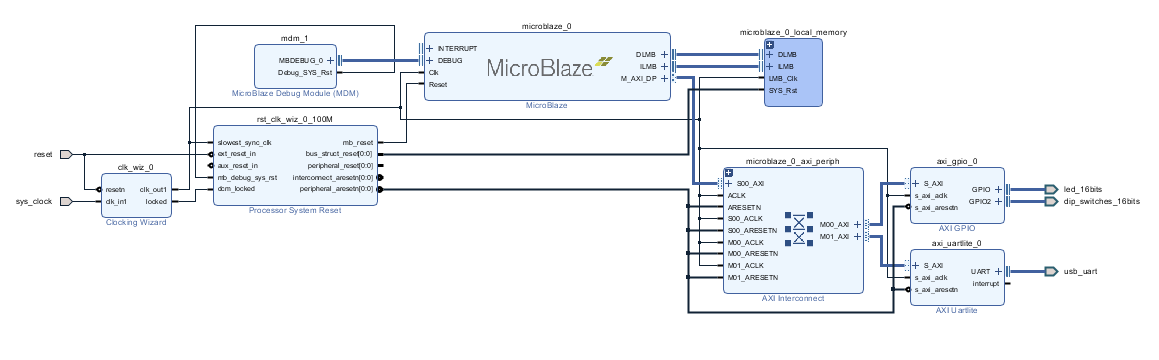
\includegraphics[width=\textwidth]{inc/block_design.PNG}

From that a VHDL wrapper can be generated and the design fully implemented. As seen below this design consumes a fair bit more resources than the previously labs smaller designs but there is still plenty of silicon left to construct the rest of a more complex deign, such as signal processing units, hardware accelerators, video processers etc that can be monitors/managed by the softcore.

\begin{center}
  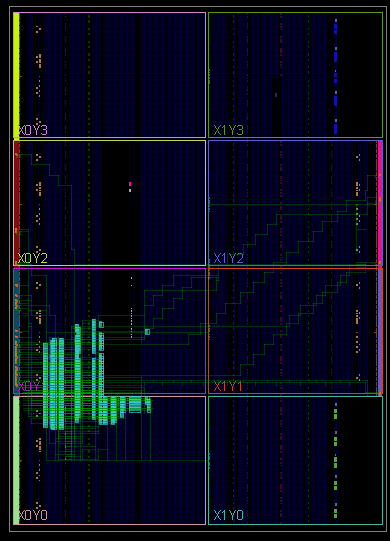
\includegraphics[width=0.3\textwidth]{inc/device.PNG}
\end{center}

From the implemented design and bitstream the project can export the hardware and Vitis can launched and setup to develop for that exports onboard MicroBlaze, for which we did the customary Hello World then made the LED's flash. 

\begin{center}
  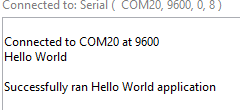
\includegraphics[]{inc/hello.PNG}
\end{center}


\end{preview}
\end{document}